\section{Module 4: Lecture 10\\Looking at rational Laplace transform and z transform together\\And\\Determining Causality of a LTI system from the system function}

\subsection{Introduction}
Till now, we have dealt with Laplace transform and z transform independently. Here, we take a look at them together and compare the procedures to get the inverse of either of them given the transforms and the regions of convergence. \\
Also, in this lecture we define the system function for continuous time and discrete time linear shift invariant systems. Further, we will learn to examine the causality of a LTI system by looking at its system function.
\subsection{System function}
The system function of a continuous independent variable LTI system is defined to be the Laplace transform of its impulse response. \\
Whereas, the system function of a discrete independent variable LTI system is define to be the z transform of its impulse response. \\
\subsection{Looking at rational Laplace transform and z transform together}
Both the rational Laplace transform and the rational z transform are associated with poles and zeroes. \\
Any rational function $p(x)/q(x)$ (where both $p(x)$ and $q(x)$ are polynomials) can be written in the following decomposed form:
\[ \frac{p(x)}{q(x)} = Quotient  +  \frac{Remainder}{Denominator} \]
\subsubsection{Quotient part}
The quotient part is a finite series in s or z depending on the transform being dealt with. For example, \\
\[ a_0 + a_1s + a_2s^2+ ... + a_ns^n + a_{-1}s^{-1} + ... + a_{-n}s^{-n} \]
\subsubsection{Laplace transform}
If the system function of a continuous independent variable LTI system has a quotient part which is anything other than a constant, the system immediately becomes unstable. (Since, e.g. an s term in the transform corresponds to differentiation and a $1/s$ term corresponds to integration).
\subsubsection{Z transform}
The quotient part of the system function of a discrete independent variable system contributes to the impulse response of the system. By itself, it can never change the stability or the instability of the system.
\subsubsection{Comparing the effect of quotient part of the system function on the stability of the system}
The quotient part of the system function of a continuous independent variable and discrete independent variable LTI system present a contrasting behavior. \\
The presence of a non constant term in the quotient part of the system function of continuous independent variable LTI system makes the system unstable. \\
Whereas, the above statement is not true for the quotient part of the z-transform. \\
This difference is to be noted. 
\subsubsection{Remainder part}
Now consider the (Remainder/Denominator) part. We can express this in terms of partial fractions. Each distinct pole which appears in the partial fraction expansion gives a “polyex” term (poly-polynomial, ex-exponential).
\subsubsection{Laplace transform}
In Laplace transform, a factor like $1/{(s-a)^M}$ with other factors in the denominator, gives a "polyex" term of the form:
\[ e^{at}*(polynomial\,\, in\,\, t\,\, of\,\, degree\,\, M-1)*(u(t)\,\, or\,\, u(-t))\, \]
Note: u(t) or u(-t) in the above expression depends on the region of convergence (ROC) of the Lapace transform.
\[ \]
We identify vertical line passing through s = a. \\ 
If the ROC is to the left of it, then we have left-sided solution. Therefore, we multiply by u(-t). \\
If the ROC is to the right of it, then we have right sided solution. Therefore, we multiply by u(t) as is already seen.
\subsubsection{Z transform}
Suppose the z transform has a term of the form $1/(1-az^{-1})^M$ multiplied by other factors in numerator and denominator. On inversion this gives a “polyex” term of the form:

\[ a^n *(a\,\, polynomial\,\, in\,\, n\,\, of\,\, degree\,\, M -1)* (u[n]\,\, or\,\, u[-n]\,\, or\,\, their\,\, shifted\,\, version)\]
where the choice between u[n] and u[-n] is based on whether the ROC is to the exterior or the interior of the circle |z|=|a|.\\
If the the ROC lies to the exterior of this circle, we have the right sided sequence (u[n]).\\
If the ROC lies inside this circle we have the left sided sequence (u[-n]).\\

An important point to note is that the region of convergence can never pass through a pole. This is because a pole is a point of singularity and so z transform or Laplace transform can never converge at a pole.
\subsubsection{Summary}
We identify the poles for the rational Laplace transform or the rational z transform as the case may be. \\
For the Laplace transform, we draw vertical lines to these poles and the possible regions of convergence are interspersed in between these vertical lines. \\
In the z transform, we draw circles centered at the origin passing through the poles and the possible regions of convergence are discs between the circles, i.e. the intervening regions between these circles.
\subsection{Illustration}
Consider the following:
\[H(z) = \frac{(1-{\frac{1}{4}}z^{-1})}{(1-2z^{-1})^2(1-{\frac{1}{3}}z^{-1})}\]
Thus we have a zero at z = ¼ and poles at z = 2 with multiplicity 2 and at z = 1/3. \\
The degree of numerator is less than the degree of the denominator and we can straight away make partial fraction expansion and invert. \\
The inverse will be of the form:
\[[(a_{10} + a_{11}n) * 2^n *(u[n]\,\, or\,\, u[-n])] + [b_{0}*({\frac{1}{3}})^n *( u[n]\,\, or\,\, u[-n])]\]
We select u[n] or u[-n] depending on the ROC.\\
\begin{figure}[h!]
	\centering
	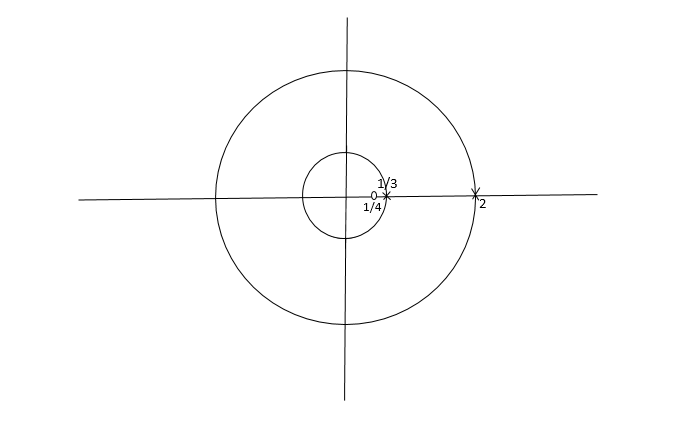
\includegraphics[width=\linewidth]{polezeroplot.png}
\end{figure}    
The pole zero plot is as shown above. We express poles by putting crosses and zeroes by circles. \\

There are 3 possible ROCs. One is inside the circle of radius 1/3(ROC1). The second one is between the 2 circles (ROC2) and the third ROC is outside both the circles (ROC3). \\
Now if an ROC is to the exterior of the circle corresponding to a pole, we choose the right sided sequence so u[n] is the choice. If ROC is in the interior of the circle corresponding to a pole, we choose the left sided sequence so u[-n] is the choice. \\

Another point to note is that there may be some loose factors in the expression of H(z) such as $z^2$. To take care of that, we need to shift u[n], in this case to u[n+2].
In case of $z^{-1}$, we would use u[n-1]. \\

ROC1:

ROC is to the interior of circles corresponding to both the poles so u[-n] for both.
So we have 
\[(a_{10}\, +\, a_{11}n) * 2^n * u[-n]\,\, +\,\, b_0*({\frac{1}{3}})^n* u[-n]\]

ROC2:

ROC is to the exterior of the circle corresponding to thepole at 1/3 and interior of the circle correspopole at 2.
So, we get
\[(a_{10}\, +\, a_{11}n) * 2^n* u[-n]\,\, +\,\, b_0*({\frac{1}{3}})^n * u[n]\]

ROC3:

ROC is to the exterior of both the poles.
So, in this case we get,
\[(a_{10}\, +\, a_{11}n) * 2^n* u[n]\,\, +\,\, b_0*({\frac{1}{3}})^n* u[n]\]
Conclusion: \\
We saw the differences and similarities in the effect of the quotient and the remainder parts of Laplace and z transforms. We also saw how the regions of convergence affect the inverse transforms of both the Laplace and z transforms.
\subsection{Determining the causality of a LTI system from its system function}
The system function of a LTI system is as complete a representation of the system as is the impulse response. Therefore, given a system function we should be able to tell if the system is causal or not. In this section, we learn methods to comment on the causality of a system given its system function for both continuous independent variable and discrete independent variable LTI systems.
\subsubsection{Relation between system function and causality of the LTI system for continuous independent variable system.}
\subsubsection{Causal system}
A continuous independent variable system is causal if its impulse response h(t) is 0 for all t<0. \\
Thus, the system function(if it exists) of a causal continuous independent variable LTI system is given by
\[ H(s) =  \int_0^\infty h(t)\, e^{-st}\, dt \]
Since s is a complex quantity, we can substitute s by ($\Sigma$ + j$\Omega$) where $\Sigma$ and $\Omega$ are real numbers.\\
Thus,
\[ H(s) =  \int_0^\infty h(t)\, e^{-({\Sigma +j\Omega })t}dt \]
\[ H(s) =  \int_0^\infty h(t)\, e^{-{\Sigma}t}\, e^{-j\Omega t}dt\]
We now need to worry about the ROC of the above Laplace transform.\\
Let us look at the integrand in the above integral. \\
The integrand is \[h(t) e^{-\Sigma t} e^{-j\Omega t}\]

The modulus of the integrand is therefore given by,\\
\[Modulus\, of\, integrand\, =  |h(t) e^{-\Sigma t} e^{-j\Omega t}|\]
\[ \quad \quad \quad \quad \quad \quad \quad \quad \quad \quad \quad \quad \quad \quad \quad \quad \quad \quad   = \, |h(t) e^{-\Sigma t}|\,\,\,\,\,\,\,\,\,\,(since\, |e^{-j\Omega t}|=1)\]                 
When $\Sigma \rightarrow \infty$, the modulus of the integrand, i.e, $|h(t) e^{-\Sigma t}| \rightarrow 0$ for all t>0.\\
The fact that we consider only positive t is a result of h(t) being zero for all t<0 (or in other words, the system being causal).\\
Since, the integrand $|h(t) e^{-\Sigma t}| \rightarrow  0$ for all t>0 when $\Sigma \rightarrow  \infty$, the Laplace transform exists(converges) at the contour $\Sigma \rightarrow \infty$.\\

Therefore, the contour $\Sigma \rightarrow \infty$ is included in the ROC of the Laplace transform of a causal system.
\subsubsection{Non-causal system}
If the system were non-causal, h(t) would have been non-zero for some negative t. This would lead to the system function 
\[ H(s) =  \int_{-\infty }^\infty h(t)\, e^{-{\Sigma}t}\, e^{-j\Omega t}dt\]
Now, if $\Sigma \rightarrow \infty$, $|h(t) e^{-\Sigma t}| \rightarrow \infty$ , for negative t. \\
Therefore, the integral also diverges at the contour  $\Sigma \rightarrow \infty $ and thus it is NOT included in the ROC.
\subsubsection{Conclusion}
A continuous independent variable LTI system is causal if and only if the contour $\Sigma \rightarrow \infty$ lies in the ROC of the system function.
\subsubsection{Relation between system function and causality of the LTI system for discrete independent variable system}
\subsubsection{Causal system}
We know that the system function of a discrete independent variable LTI system is the z transform(if it exists) of the impulse response. \\
A continuous independent variable system is causal if its impulse response h[n] is 0 for all n<0. \\
Thus, the system function of a causal discrete independent variable LTI system is given by
\[ H(z) = \sum_{0}^{\infty } \, h[n]z^{-n} \]
We now need to worry about the ROC of the above z transform.\\
Let us look at the summand in the above summation.\\ 
The summand is
\[ h[n] z^{-n} \]
The modulus of the summand is therefore given by,
\[Modulus\, of\, summand =  |h[n] z^{-n}|\]
\[ \quad \quad \quad \quad \quad \quad \quad \quad \quad \quad \quad       = \, |h[n]|\,|z|^{-n} \]\\

The modulus of the summand, $|h[n]|\, |z|^{-n} \rightarrow 0$ for all n>0 and,
is equal to $|h[n]|$ for n=0. \\
Thus, the z transform also exists(converges) at the contour $|z| \rightarrow \infty $ \\
The fact that we consider only non-negative n is a result of h[n] being zero for all n<0 (or in other words, the system being causal). \\

Therefore, the contour $|z| \rightarrow \infty $ is included in the ROC of the z transform of a causal system. Loosely speaking this contour is the outermost circle in the z plane.
\subsubsection{Non causal system}
If the system were non-causal, h[n] would have been non-zero for some negative n. This would lead to the system function 
\[ H(z) = \sum_{-\infty }^{\infty } \, h[n]z^{-n} \]
Now, if $|z| \rightarrow \infty $, the summand $|h[n]|\,|z|^{-n} \rightarrow \infty $, for negative n. 
Therefore, the summation also diverges at the contour $ |z| \rightarrow \infty $ and thus it is NOT included in the ROC.

\subsubsection{Conclusion}
A discrete independent variable LTI system is causal if and only if the contour $|z| \rightarrow \infty $ lies in the ROC of the system function.
